\begin{figure}[t]
\centering
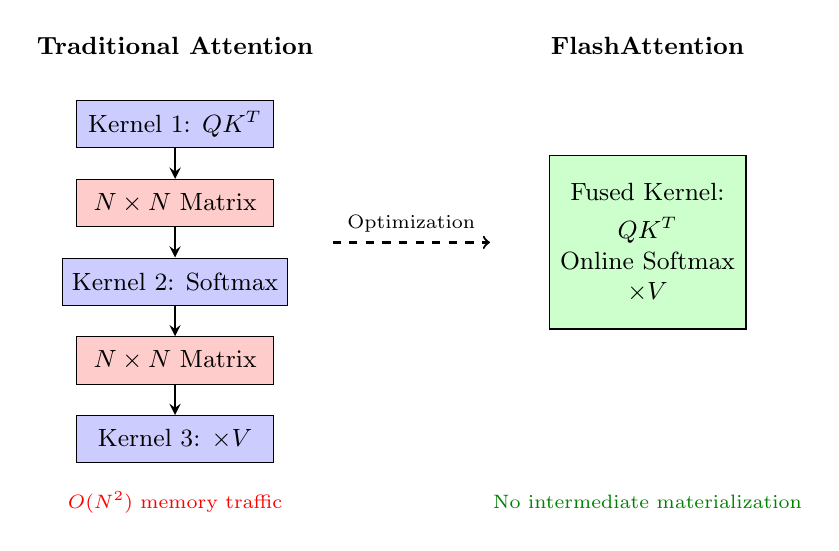
\begin{tikzpicture}[
    kernel/.style={rectangle, draw, fill=blue!20, minimum width=2.5cm, minimum height=0.6cm, font=\small},
    memory/.style={rectangle, draw, fill=red!20, minimum width=2.5cm, minimum height=0.6cm, font=\small},
    fused/.style={rectangle, draw, fill=green!20, minimum width=2.5cm, minimum height=2.2cm, font=\small, align=center},
    arrow/.style={->, >=stealth, thick}
]

% Traditional Attention (Left)
\node[font=\small\bfseries] at (-3, 2.5) {Traditional Attention};

\node[kernel] (qk) at (-3, 1.5) {Kernel 1: $QK^T$};
\node[memory] (mat) at (-3, 0.5) {$N \times N$ Matrix};
\node[kernel] (sm) at (-3, -0.5) {Kernel 2: Softmax};
\node[memory] (mat2) at (-3, -1.5) {$N \times N$ Matrix};
\node[kernel] (mul) at (-3, -2.5) {Kernel 3: $\times V$};

\draw[arrow] (qk) -- (mat);
\draw[arrow] (mat) -- (sm);
\draw[arrow] (sm) -- (mat2);
\draw[arrow] (mat2) -- (mul);

\node[font=\scriptsize, text=red] at (-3, -3.3) {$O(N^2)$ memory traffic};

% FlashAttention (Right)
\node[font=\small\bfseries] at (3, 2.5) {FlashAttention};

\node[fused] (flash) at (3, 0) {
    Fused Kernel:\\[0.1cm]
    $QK^T$ \\
    Online Softmax \\
    $\times V$
};

\node[font=\scriptsize, text=green!50!black] at (3, -3.3) {No intermediate materialization};

% Arrow between two approaches
\draw[->, dashed, thick] (-1, 0) -- (1, 0) node[midway, above, font=\scriptsize] {Optimization};

\end{tikzpicture}
\caption{Comparison between traditional Attention and FlashAttention. Traditional approach requires three separate kernels and materializes $N \times N$ attention matrices in global memory, while FlashAttention fuses all operations with online softmax, eliminating memory bottlenecks.}
\label{fig:attention_comparison}
\end{figure}
